\documentclass[10pt,twoside]{article}

\usepackage[T1]{fontenc}
\usepackage[utf8]{inputenc}
\usepackage{newtxtext}
\usepackage{mathtools,amsthm}
\usepackage{newtxmath}
\usepackage[margin=0.78in,top=0.62in,bottom=0.70in]{geometry}
\usepackage{microtype}
\usepackage{xcolor}
\usepackage{booktabs,tabularx,array}
\usepackage{enumitem}
\usepackage{titlesec}
\usepackage{caption}
\usepackage{float}
\usepackage{tikz}
\usepackage{pgfplots}
\usepackage[numbers,sort&compress]{natbib}
\usepackage[colorlinks=true,allcolors=MidnightBlue]{hyperref}
\usepackage[nameinlink,noabbrev]{cleveref}

\pgfplotsset{compat=1.18}

\definecolor{MidnightBlue}{HTML}{16324F}
\definecolor{SignalBlue}{HTML}{277DA1}
\definecolor{WarmGold}{HTML}{D69E2E}
\definecolor{SoftRed}{HTML}{C8553D}
\definecolor{Forest}{HTML}{3D7A62}
\definecolor{Ink}{HTML}{20262E}
\definecolor{Mist}{HTML}{F2F5F7}
\definecolor{RuleGray}{HTML}{CBD5DE}

\color{Ink}
\hypersetup{pdfauthor={Jonathan R. Landers},pdftitle={The Shape of What Remains}}
\setlength{\parindent}{1.05em}
\setlength{\parskip}{0.12em}
\setlist{nosep,leftmargin=1.35em}
\captionsetup{font=small,labelfont={bf,color=MidnightBlue},skip=4pt}
\titleformat{\section}{\Large\bfseries\color{MidnightBlue}}{}{0pt}{}
\titleformat{\subsection}{\large\bfseries\color{MidnightBlue}}{}{0pt}{}
\titlespacing*{\section}{0pt}{1.05em}{0.36em}
\titlespacing*{\subsection}{0pt}{0.78em}{0.24em}
\pagestyle{plain}

\newtheoremstyle{noteplain}
  {0.58em}{0.58em}{\itshape}{} {\bfseries\color{MidnightBlue}}{.}{0.5em}{}
\theoremstyle{noteplain}
\newtheorem{theorem}{Theorem}
\newtheorem{lemma}[theorem]{Lemma}
\newtheorem{proposition}[theorem]{Proposition}
\theoremstyle{definition}
\newtheorem{definition}[theorem]{Definition}
\renewcommand{\qedsymbol}{\color{SignalBlue}$\blacksquare$}

\newcommand{\E}{\mathbb{E}}
\newcommand{\Prb}{\mathbb{P}}
\newcommand{\F}{\mathcal{F}}
\newcommand{\takeaway}[1]{%
  \par\medskip
  \noindent\fcolorbox{SignalBlue}{Mist}{%
    \begin{minipage}{0.94\linewidth}
      \small\textbf{Takeaway.} #1
    \end{minipage}}
  \par\medskip
}

\begin{document}

\begin{center}
  {\fontsize{25}{29}\selectfont\bfseries\color{MidnightBlue}The Shape of What Remains}\par\vspace{0.25em}
  {\Large Regional prediction from partial Hadamard constraints}\par\vspace{0.85em}
  {\normalsize Jonathan R. Landers}\par\vspace{0.25em}
  {\small August 2026}
\end{center}

\vspace{0.35em}
\noindent\colorbox{Mist}{%
\begin{minipage}{0.965\linewidth}
\small
\textbf{Abstract.}
A Hadamard matrix is exactly constrained as a whole, yet its next serialized entry need not be predictably nonrandom under equivalent presentations.  We ask whether the wrong local object has been predicted.  For a partially exposed row, balance fixes the remaining sign inventory and each partial inner product fixes the remaining agreement inventory with a completed row.  Under randomized coordinate order these inventories induce exact hypergeometric laws for next-block composition.  On held-out equivalence classes of orders $24$ and $28$, those state laws predict regional summaries at block sizes $2,4,8$, including early in construction, while serialized context adds no residual gain after representation randomization.  We then enumerate every immediately feasible block at ambiguous nonterminal states.  At order $28$ and block size $8$, a composite score over all prior-row constraints ranks the observed valid continuation at the $84.8$th percentile early and the $93.2$nd percentile mid-construction, versus the $50$th percentile for random order.  Global rigidity is therefore locally visible---not primarily as the next sign, but as the shape of the correction that remains.  This supplies a theorem-backed branch-ordering candidate for exact search without turning preference into pruning.
\end{minipage}}

\section{The local object was hiding in the state}

A Hadamard matrix $H\in\{-1,+1\}^{d\times d}$ satisfies
\begin{equation}\label{eq:hadamard}
HH^{\mathsf T}=dI_d.
\end{equation}
Its rows are not merely balanced; every pair is perfectly coordinated.  Yet the preceding note found that a short row-wise context predicts held-out catalog representatives far better than equivalent matrices whose rows and columns have been randomly permuted.  Most serialized predictability follows the representative rather than the equivalence class.

That negative result changes the question.  Arbitrary adjacency is not intrinsic under Hadamard equivalence, but an exact constructor does possess an intrinsic local object: its evolving constraint state.  After a partial assignment, the solver knows how much row imbalance and pairwise correlation remain to be repaired.  Individual signs may remain interchangeable while a region has a sharply constrained composition.

This note closes that conceptual loop.  It first localizes the catalog signal to within-sequence coordinate order.  It then derives regional probability laws from partial balance and orthogonality, verifies them across randomized equivalent presentations, and asks the search-facing question: do those laws rank ambiguous candidate blocks?

The resulting project sentence is:
\begin{quote}
\centering\itshape
Hadamard matrices are globally choreographed, locally elusive entry by entry, yet regionally predictable through their evolving constraint state---structure that may guide an exact search.
\end{quote}

Hadamard equivalence, normalization, and classification are classical \citep{horadam2007,spence1995}.  We use the McKay equivalence-class corpus \citep{mckaydata}; probability forecasts are evaluated by held-out logarithmic loss, a strictly proper score \citep{gneitingraftery2007}.  The contribution is not a new classification or a claim that rows are Markov chains.  It is a change of coordinates on the prediction problem: from the last few printed symbols to the amount of exact correction still owed.

\section{From representation diagnosis to correction laws}

\subsection{Why the serialized signal moves}

We normalize the first row and column to $+1$.  A row-reset length-$k$ observation never crosses a row boundary.  Its counts are sums of within-row substring counts, which gives an exact negative control.

\begin{lemma}[Pooling invariance]\label{lem:pooling}
For row-reset traversal, permuting whole rows leaves every context/target count unchanged.  Dually, permuting whole columns leaves every column-reset count unchanged.  An opposite-axis permutation may change either statistic by changing coordinate adjacency within each sequence.
\end{lemma}

\begin{proof}
Whole-row permutation only reorders the summands in the pooled row count.  Column permutation reorders coordinates inside every row and need not preserve substrings.  Transposition gives the dual statement.
\end{proof}

The paired experiment uses $20$ class-level splits at orders $24$ and $28$, lengths $k=1,\ldots,12$, catalog representatives, fixed-anchor permutations of either or both axes, unrestricted permutations followed by renormalization, both traversals, and removal of either normalization anchor.  All $40$ source-split leakage audits pass.

At $k=8$, column permutation lowers row-reset catalog gain by $0.13361$ nats per sign at order $24$ and $0.10895$ at order $28$; row permutation changes it by less than $4\times10^{-17}$.  The exact dual holds for column traversal.  Strict-interior prediction retains $0.15113$ and $0.11929$ nats at orders $24$ and $28$, so normalization is not the main source.  The signal lives in within-sequence coordinate order.

\subsection{What the unfinished region must contain}

Now construct normalized nonfirst row $i$ from left to right.  After $m$ entries, define
\begin{equation}\label{eq:state}
R_i(m)=\sum_{\ell=1}^{m}H_{i\ell},
\qquad
S_{ij}(m)=\sum_{\ell=1}^{m}H_{i\ell}H_{j\ell},
\qquad
r=d-m.
\end{equation}
Because row $i$ is balanced and orthogonal to every earlier row $j$,
\begin{equation}\label{eq:debts}
\sum_{\ell=m+1}^{d}H_{i\ell}=-R_i(m),
\qquad
\sum_{\ell=m+1}^{d}H_{i\ell}H_{j\ell}=-S_{ij}(m).
\end{equation}

\begin{theorem}[Regional correction law]\label{thm:regional}
Let the remaining $r$ coordinates of a completed Hadamard row be exposed in uniformly random order.  The number $Y_b$ of plus signs in the next $b\le r$ positions has distribution
\begin{equation}\label{eq:row-hyper}
\Prb(Y_b=q\mid R_i(m))
=\frac{\binom{P_i(m)}q\binom{r-P_i(m)}{b-q}}{\binom rb},
\qquad
P_i(m)=\frac{r-R_i(m)}2.
\end{equation}
For any completed row $j<i$, the number $Z_{b,j}$ of agreements in the block has marginal distribution
\begin{equation}\label{eq:pair-hyper}
\Prb(Z_{b,j}=q\mid S_{ij}(m))
=\frac{\binom{A_{ij}(m)}q\binom{r-A_{ij}(m)}{b-q}}{\binom rb},
\qquad
A_{ij}(m)=\frac{r-S_{ij}(m)}2.
\end{equation}
\end{theorem}

\begin{proof}
If $P$ of $r$ remaining objects are marked, a uniformly selected ordered block of size $b$ contains $q$ marked objects with the hypergeometric probability in \eqref{eq:row-hyper}.  Equation \eqref{eq:debts} gives $P=P_i(m)$.  Apply the same counting argument to the remaining products $H_{i\ell}H_{j\ell}$, marking agreements, to obtain \eqref{eq:pair-hyper}.  Each pairwise law is marginal; the laws for different $j$ are not asserted independent.
\end{proof}

The expectation makes the direction transparent:
\begin{equation}\label{eq:expectations}
\E[Y_b\mid R_i(m)]=\frac{bP_i(m)}r,
\qquad
\E[2Z_{b,j}-b\mid S_{ij}(m)]=-\frac{bS_{ij}(m)}r.
\end{equation}
A positive partial inner product therefore predicts a negatively aligned regional correction.  Global choreography points locally, but toward a block composition rather than necessarily toward one entry.

\takeaway{The theorem is representation-resilient rather than tied to one catalog order: after any equivalent presentation is chosen, the current state recomputes the exact inventory that its remaining coordinates must spend.}

\section{Regional forecasts survive random presentation}

The regional study uses all $60$ order-$24$ and $487$ order-$28$ catalog classes, $20$ paired $80/20$ splits, block sizes $b\in\{2,4,8\}$, and three presentations: catalog, fixed-anchor randomization of both axes, and unrestricted randomization followed by renormalization.  Every split passes the index/digest audit.

We predict two categorical targets: the next-block plus count $Y_b$, and $Z_{b,j^*}$ for the previous nonfirst row
\begin{equation}
j^*\in\arg\max_{1\le j<i}|S_{ij}(m)|,
\end{equation}
the pair under greatest current pressure.  Four models are compared: a fair binomial block, a smoothed length-$4$ serialized-context table using the Krichevsky--Trofimov pseudocount \citep{krichevskytrofimov1981}, the exact state law in \cref{thm:regional}, and a context table shrunk toward that law.  Early, middle, and late stages are reported separately using thirds of $m/d$.  Intervals bootstrap the $20$ repetition means with $10{,}000$ resamples.

\begin{table}[t]
\centering
\caption{Constraint-state gain over fair block guessing under unrestricted permutation and renormalization, $b=8$, in held-out nats per block.}
\label{tab:regional}
\small
\begin{tabular}{@{}clccc@{}}
\toprule
$d$ & Target & Early & Middle & Late \\
\midrule
24 & row composition & $0.0851$ & $0.3851$ & $1.6163$ \\
24 & pressured-pair agreement & $0.1670$ & $0.9018$ & $2.5025$ \\
28 & row composition & $0.0572$ & $0.2014$ & $1.6379$ \\
28 & pressured-pair agreement & $0.1201$ & $0.5462$ & $2.6659$ \\
\bottomrule
\end{tabular}
\end{table}

Every early-stage interval is above zero for both targets, every $b$, and both orders.  For example, the order-$28$, $b=8$ pressured-pair interval is $[0.11727,0.12273]$ early and $[0.54202,0.54999]$ middle.  The fixed-anchor presentation is nearly identical.  Late prediction becomes strong because the correction inventory is nearly spent, but \cref{tab:regional} shows that the effect is present well before completion.

Serialized context contributes no residual gain after randomization.  At order $28$, $b=8$, state-plus-context is worse than state alone by $0.00337$ nats early and $0.02004$ middle for pressured-pair agreement.  In catalog order it adds $0.17693$ and $0.39279$ nats.  The experiments therefore separate two signals cleanly:
\begin{equation}\label{eq:separation}
\underbrace{\text{state correction}}_{\text{survives representation randomization}}
\qquad+\qquad
\underbrace{\text{serialized residual}}_{\text{catalog-order specific}}.
\end{equation}

\section{Does the state know which block to try?}

Prediction becomes search guidance only if it distinguishes continuations.  At sampled early and middle states, we enumerate every $x\in\{-1,+1\}^b$ and retain the immediately feasible set $\F_b$: after assigning $x$, row balance and every pair must still satisfy
\begin{equation}\label{eq:feasible}
|R_i(m+b)|\le r-b,
\qquad
|S_{ij}(m+b)|\le r-b.
\end{equation}
Terminal states and states with $|\F_b|=1$ are excluded.

For candidate $x$, let $q_0(x)$ be its plus count and $q_j(x)$ its agreement count with row $j$.  The all-pair score is
\begin{equation}\label{eq:score}
L_{\mathrm{all}}(x)
=\log\Prb(Y_b=q_0(x)\mid R_i(m))
+\sum_{1\le j<i}\log\Prb(Z_{b,j}=q_j(x)\mid S_{ij}(m)).
\end{equation}
This is a composite likelihood used only for ranking; the pairwise targets are dependent.  We compare random order, balance alone, balance plus a random pair, balance plus $j^*$, all-pair score, and minimizing the worst absolute post-block pressure.  Each repetition samples at most $500$ ambiguous states per order, block size, stage, and presentation.  The primary metric is the tie-aware percentile of the observed valid continuation inside $\F_b$; random ordering is $0.5$.

\begin{table}[H]
\centering
\caption{Offline ranking after unrestricted permutation and renormalization, $b=8$.  ``Top 10'' is the fraction of observed valid blocks in the highest candidate decile.}
\label{tab:ranking}
\small
\begin{tabular}{@{}clcccc@{}}
\toprule
$d$ & Stage & Balance & Pressured pair & All pairs & Top 10 \\
\midrule
24 & early  & $0.583$ & $0.654$ & $0.876$ & $0.644$ \\
24 & middle & $0.622$ & $0.651$ & $0.859$ & $0.737$ \\
28 & early  & $0.563$ & $0.621$ & $0.848$ & $0.586$ \\
28 & middle & $0.627$ & $0.732$ & $0.932$ & $0.800$ \\
\bottomrule
\end{tabular}
\end{table}

The all-pair intervals are narrow: $[0.8447,0.8515]$ early and $[0.9293,0.9339]$ middle at order $28$.  The effect persists for every $b$ in \cref{fig:ranking}.  At order $28$, $b=8$, the minimum-worst-pressure heuristic reaches $0.736$ early and $0.866$ middle, materially below $L_{\mathrm{all}}$.  Balance is useful, one pair adds information, and combining all orthogonality obligations is decisively stronger.  Regional guidance is not row balance in disguise.

\begin{figure}[t]
\centering
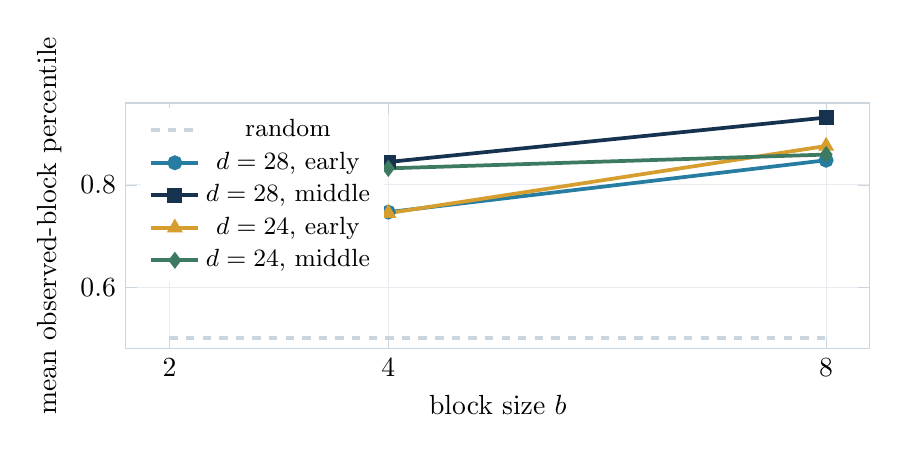
\begin{tikzpicture}
\begin{axis}[
  width=0.91\linewidth,
  height=4.7cm,
  xmin=1.6,xmax=8.4,
  ymin=0.48,ymax=0.96,
  xtick={2,4,8},
  xlabel={block size $b$},
  ylabel={mean observed-block percentile},
  axis line style={draw=RuleGray},
  tick style={draw=RuleGray},
  grid=major,
  grid style={draw=RuleGray!45},
  legend style={draw=none,fill=white,font=\small,at={(0.02,0.98)},anchor=north west},
  every axis plot/.append style={line width=1.35pt,mark size=2pt}
]
\addplot[color=RuleGray,dashed,domain=2:8] {0.5};
\addlegendentry{random}
\addplot[color=SignalBlue,mark=*] coordinates {(2,0.6542) (4,0.7467) (8,0.8481)};
\addlegendentry{$d=28$, early}
\addplot[color=MidnightBlue,mark=square*] coordinates {(2,0.7384) (4,0.8447) (8,0.9316)};
\addlegendentry{$d=28$, middle}
\addplot[color=WarmGold,mark=triangle*] coordinates {(2,0.6602) (4,0.7447) (8,0.8760)};
\addlegendentry{$d=24$, early}
\addplot[color=Forest,mark=diamond*] coordinates {(2,0.7307) (4,0.8322) (8,0.8592)};
\addlegendentry{$d=24$, middle}
\end{axis}
\end{tikzpicture}
\caption{All-pair ranking under unrestricted equivalent randomization.  Every point is computed only on ambiguous nonterminal states.}
\label{fig:ranking}
\end{figure}

\takeaway{A solver can calculate the score from its current exact state, and the score strongly prefers the continuation found in held-out valid matrices.  This is the first empirical bridge from global structure to local search action.}

\section{What the evidence establishes}

The apparent contradiction is resolved.  Global structure need not make the next arbitrary coordinate predictable; a parity-constrained sequence can have uniform small marginals while its final sign is forced.  Hadamard constraints similarly act through inventories spread across the unfinished region.  Serialized windows miss most invariant information, while $R_i(m)$ and the vector $(S_{ij}(m))_{j<i}$ expose how the region must compensate.

The result is stronger than the first note's catalog effect in one sense and weaker in another.  It survives randomized equivalent presentations and is mathematically interpretable.  But \cref{thm:regional} is exact for uniformly reordered remaining coordinates, not a theorem that the unfinished part of every solver state is uniformly distributed over Hadamard completions.  Likewise, \eqref{eq:score} is a useful composite ranking, not a joint probability model.

Most importantly, the observed block is only one continuation from a known complete matrix.  A highly ranked counterfactual block may pass \eqref{eq:feasible} yet admit no full completion.  Offline percentile does not equal first-solution speedup.  The next note must embed $L_{\mathrm{all}}$ in a complete solver, hold exact pruning fixed, and compare nodes and backtracks with random, lexicographic, balance-only, and minimum-pressure orderings.  Statistical scores may reorder feasible branches; they may not delete one.

The evidence also remains finite: two orders, one fixed corpus, and repeated class-level splits rather than a population sample of all Hadamard matrices.  Bootstrap intervals quantify split and representation randomization for that corpus.  They do not establish an asymptotic law.

\section{Conclusion}

The strong serialized signal lived in the representative.  The stronger structural lesson lives elsewhere: in the debt carried by an unfinished region.  Balance determines how many signs remain; orthogonality determines how many agreements remain; together those debts predict block composition under arbitrary equivalent presentations.  When combined across prior rows, they also rank ambiguous valid continuations far above random.

Thus global choreography does point locally, but its pointing device is not the last few symbols.  It is the evolving constraint state.  The exact-solver experiment now has a principled policy to test and a clean failure condition: if this ranking does not reduce first-solution work, the predictive and algorithmic stories should separate.  If it does, the narrative closes from global law, through regional information, to exact construction.

\paragraph{Reproducibility.}
The repository contains exact corpus verification; all three paired experiments; $120$ passing split audits; $23{,}520$ raw measurements; bootstrap summaries; environment metadata; candidate enumeration and exact feasibility checks; and unit tests for the regional laws and tie-aware ranking.  Raw source downloads remain regenerable from the cited catalog.

\bibliographystyle{plainnat}
\bibliography{references}

\end{document}
